\documentclass[12pt,a4paper]{article}

\usepackage[utf8]{inputenc}
\usepackage[ngerman]{babel}
\usepackage[T1]{fontenc}
\usepackage{amsmath}
\usepackage{amsfonts}
\usepackage{amssymb}
\usepackage{graphicx}
\usepackage[left=2cm,right=2cm,top=2cm,bottom=2cm]{geometry}
\usepackage{multicol}
\usepackage{booktabs}
\usepackage[hidelinks]{hyperref}
\usepackage{tikz}
\usepackage{pgfplots}
\usepackage{blindtext}
\usepackage{array}
\usepackage{multirow}
\usepackage{bigdelim}
\usepackage{colortbl}
\usepackage{fancyhdr} 
\usepackage{tabularx}
\usepackage{xcolor}
\usepackage{color}
\usetikzlibrary{decorations.text}
\usetikzlibrary{tikzmark}
\pagestyle{fancy} 
	\fancyhf{} 
	\fancyhead[L]{
\includegraphics[scale=0.05]{Bilder/dhbw.png}} 
	\fancyhead[C]{\slshape Netztechnik} 
	\fancyhead[R]{\slshape LaTeX Version}
	\fancyfoot[C]{\thepage}
\usepackage{helvet}
\renewcommand{\familydefault}{\sfdefault}

\title{Netztechnik}
\author{\slshape Robin Rausch, Florian Maslowski}
\date{\slshape \today}

\begin{document}
	\pagenumbering{Roman}
	\maketitle
	\tableofcontents
	\newpage
	\pagenumbering{arabic}
	\section{Grundlagen}
		\subsection{OSI-7-Schichten-Modell}
			\textbf{Merkhilfe:} Please Do Not Throw Salami Pizza Away.\\
			Zweck des Open-System-Interconnection-Modells ist, Kommunikation über unterschiedlichste technische Systeme hinweg zu beschreiben und die Weiterentwicklung zu begünstigen.\newline\newline
			\begin{minipage}{.5\textwidth}
				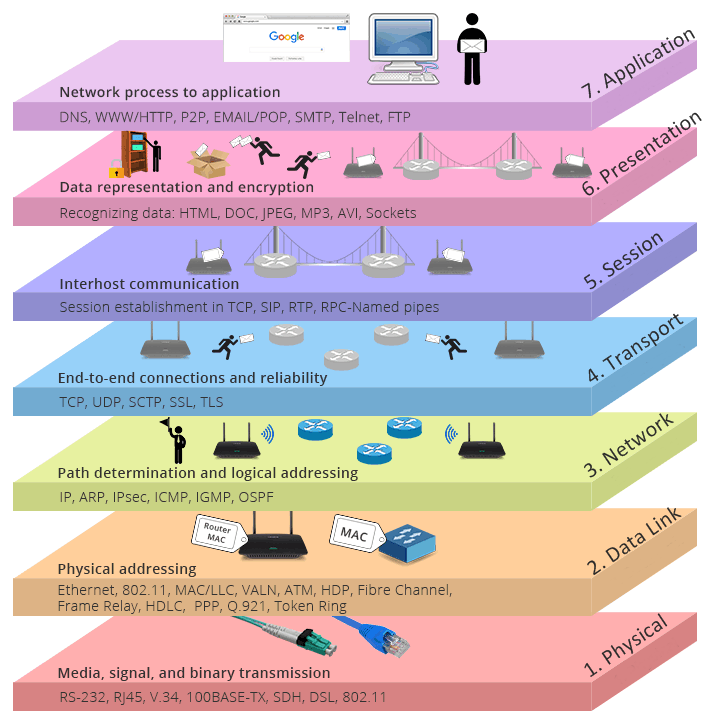
\includegraphics[scale=.45]{Bilder/OSI-Modell1} %aus Abi-Lernzettel kopiert
			\end{minipage}
			\begin{minipage}{.5\textwidth}
				\textbf{Hauptaufgaben der Schichten:}
				\begin{itemize}
					\item Schicht 7: Anwendungen für Benutzer
					\item Schicht 6: Darstellung der Daten in verständliche Formate (jpg, ASCII)
					\item Schicht 5: Steuerung der Verbindung
					\item Schicht 4: Zuordnung der Datenpakete zu den Ports
					\item Schicht 3: Vermittelt Datenpakete
					\item Schicht 2: Fehlerfreie Übertragung
					\item Schicht 1: Bit-Übertragung 
				\end{itemize}
			\end{minipage}
			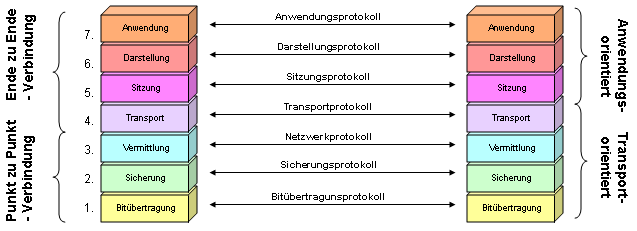
\includegraphics[scale=.75]{Bilder/OSI-Modell2} %aus Abi-Lernzettel kopiert

		\subsection{Protokolle (+Zuordnung)}
			\subsubsection{Layer 1: Physical Layer - Bitübertragungsschicht}
				Diese Schicht beschreibt die physische Übertragung der Daten. Zusammenfassend geht es hierbei hauptsächlich um Kabel und Sender/Empfänger. \textcolor{red}{??}

			\subsubsection{Layer 2: Data Link Layer - Sicherungsschicht}
				Hier wird der Ethernet Frame zusammengebaut und NIC und MAC-Adressen verwendet. Die MAC-Adresse fällt deshalb auch unter die Schicht 2 und wird später genauer erklärt. \textcolor{red}{??}

			\subsubsection{Layer 3: Network-Layer - Vermittlungsschicht}
				Die Schicht 3 beschreibt das Routing in einem Netzwerk. Darunter fallen beispielsweise Switches. \textcolor{red}{??}

			\subsubsection{Layer 4: Transport Layer - Transportschicht}
				Layer 4 stellt eine transparente Datenübertragung zwischen Endsystemen zur Verfügung. Darunter fallen beispielsweise TCP und UDP:\newline\newline
				Bei TCP wird vor dem Datentransport eine Verbindung zwischen den Parteien aufgebaut und während des gesamten Datenaustausches gehalten. Nach Abschluss des Datenflusses wird die Verbindung wieder abgebaut. Verwendet werden hierbei Timer, Wiederholungen, FLusskontrolle, Windowing/Stop and Wait und Multiplexing um eine Verbindung mehrfach nutzen zu können.\newline\newline
				Bei UDP werden die Daten in das Netzwerk in Richtung Empfänger gesendet, ohne dass der Sender weiß, ob der Empfänger empfangsbereit ist. Damit sind die oben aufgeführten Mechanismen, wie Flusskontrolle und Wiederholungen in den überlagerten Schichten zu bearbeiten.

			\subsubsection{Layer 5: Session Layer - Sitzungsschicht}
				Diese Schicht ist die erste anwendungsorientierte Schicht und behandelt Sitzungsabläufe und Synchronisationspunkte. Wenn ein Fehler auftritt, kann auf diese Synchronisationspunkte aufgesetzt werden. Ebenso fallen die Betriebsarten(Simplex, Half-Duplex und Full-Duplex) und Phasen(Verbindungsaufbau, Datenübertragung und Verbindungsaufbau) unter diese Schicht. \textcolor{red}{??}

			\subsubsection{Layer 6: Presentation Layer - Darstellungsschicht}
				Unterschiedliche Rechner haben aufgrund unterschiedlicher Betriebssysteme unterschiedliche Darstellungsformen der Daten. Soll eine Applikation auf unterschiedlichen Betriebssystemen ablaufen können, sind Konvertierungen durchzuführen.
				Hier werden folgende Umsetzungen abgewickelt:\newline
				Zeichensätze (ASCII, EBCDIC), Interpretation von Bytes MSB (Most Significant Bit)/LSB (Least Significant Bit), Kompression/Dekompression und Verschlüsselung/Entschlüsselung

			\subsubsection{Layer 7: Application Layer - Anwendungsschicht}
			Diese Schicht bildet die Schnittstelle zum Anwender (User). Beispiel hierfür sind:\newline
			FTP File Transfer Protocol, SMTP Simple Mail Transfer Protocol, SNMP Simple Network Management Protocol und DNS Domain Name Service

	\section{MAC-Adresse}
	Die MAC-Adresse gehört zur OSI Schicht 2 und besteht aus 48bit welche in 4 Teile eingeteilt werden:
	\begin{center}
		\begin{figure}
			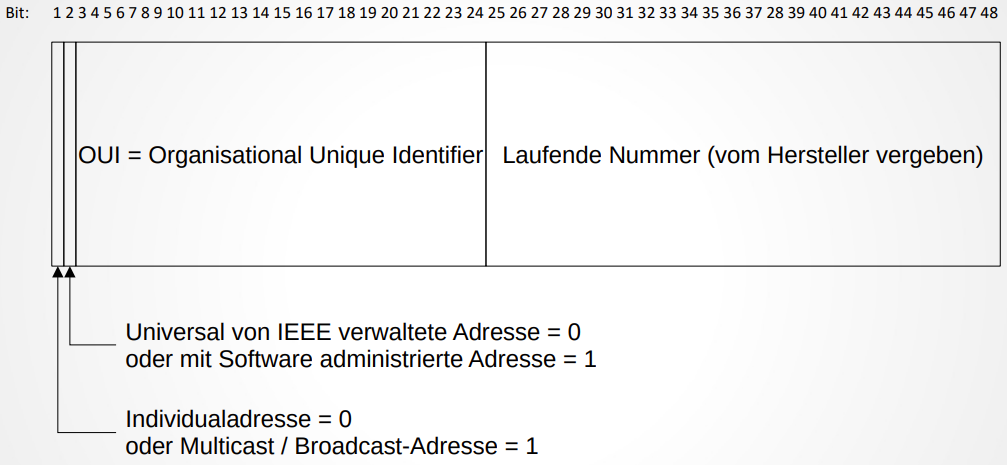
\includegraphics[width=\textwidth]{Bilder/MAC-Adresse.PNG}
		\end{figure}
	\end{center}

	\section{Netze}
		\subsection{Netzwerk-Topologien}

		\subsection{Netzwerk-Technologien}
			\begin{description}
				\item[Repeater] Verstärkt Eingangssignal auf Ausgang, OSI-Schicht 1
				\item[Hub] Multiport Repeater, OSI-Schicht 1
				\item[Bridge] Verbindet 2 Netze, arbeitet mit MAC-Adressen, OSI-Schicht 2 
				\item[Switch] Schlauer Hub. Verstärkt nur an richtigen Port. Arbeitet mit MAC-Adressen, OSI-Schicht 2 
				\item[Router] Verbindet Netze, arbeitet mit IP-Adressen, OSI-Schicht 3
				\item[Gateway] Verbindet Netze, arbeitet auf allen OSI-Schichten, Protokollunabhängig 
			\end{description}

		\subsection{Subnetting}

		\subsection{Switch}
			\subsubsection{Spanning Tree}
				Switche haben Hierarchie beim Weiterleiten von Paketen. Kleine Priorität ist besser. Falls Priorität gleich, entscheidet höhere MAC-Adresse die bevorzugte Switch\\
				Switche geben Pakete nur an Switche mit geringerer Priorität oder höherer MAC-Adresse weiter. Beste Switch in der Vernetzung wird zum Root.\\
				Es gibt dabei 3 Arten von Ports an den Switches:
				\begin{description}
					\item[Root-Port] Zur Root-Switch
					\item[Designated-Port] Zu Switch mit besserer Priorität oder höherer MAC-Adresse als die eigene
					\item[Blocking-Port] Zu Switches, welche weniger bevorzugt sind als sie selbst 
				\end{description}
				In Untenstehender Skizze ist Switch B die Root-Switch und alle Ports, die zu ihr führen, sind Root-Ports.\\
				Da die restlichen Switche die gleiche Priorität haben, wird die höchste MAC-Adresse bevorzugt. \\
				Dadurch sind die Ports zu Switch A die Blocking-Ports und die von D zu A und C ebenfalls. \\
				Ports an Root-Switch sind alle designated.\\
				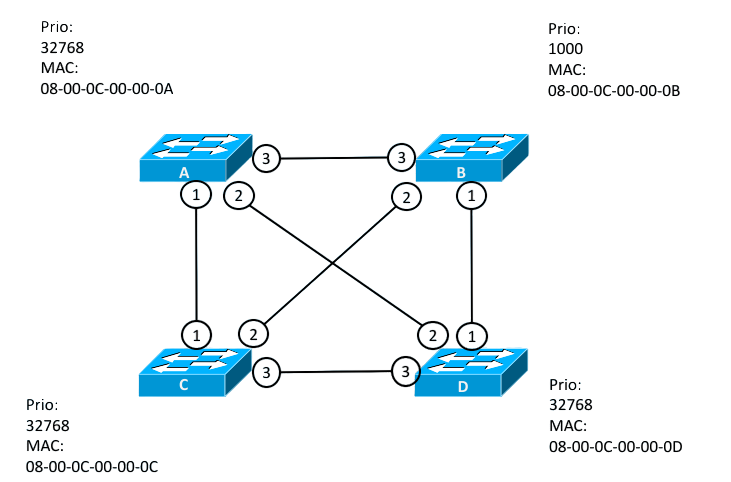
\includegraphics[scale=0.5]{Bilder/RouterVermascht.png}

	\section{Kabel}

		\subsection{Kabelarten:}
		\begin{description}
			\item[Twisted-Pair] Verdrillte Paare, um geringes Nebensprechen mit hoher Übertragbarkeit zu erreichen.
			\item[LWL] Lichtwellenleiter/Glasfaserkabel hohe Geschwindigkeit, teuer, Aufwand in Spannung zurückzuwandeln.
		\end{description}

		\subsection{Verkablungsarten:}
		\begin{description}
			\item[Primarverkabelung: ] Für Verkabelung von Gebäuden mit LWL
			\item[Sekundärverkabelung: ] Für Verkabelung von Etagen mit LWL
			\item[Tertiärverkabelung: ] Für Verkabelung innerhalb einer Etage mit Kupferkabel
		\end{description}

	\section{Codierung}
		\subsection{Huffmann-Codierung}
			Algorythmus zum \textbf{Komprimieren} von Dateien.\\
			\textbf{Idee:} Häufige Zeichen kurze Bit-Codierung, sodass Binär-Codierung möglichst kurz ist.
			\begin{enumerate}
				\item \textbf{Tabelle} mit vorkommenden Zeichen und deren Häuffigkeit erstellen
				\item \textbf{Binärbaum} mit Zeichen erstellen. Zeichen nach Häufigkeit sortiert. Zeichen mit geringster Häufigkeit zusammenfassen. Zusammengefasste zeichen weiter vereinen bis Baum vollständig ist\\
				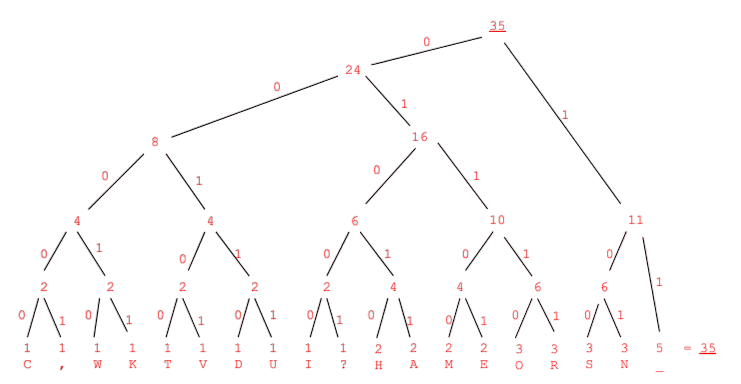
\includegraphics[scale=0.4]{Bilder/Huffmann-Baum.png}
				\item \textbf{Codierung} der Zeichen aus Binärbaum lesen und in Tabelle schreiben
			\end{enumerate}
\end{document}
